\documentclass[a4paper]{article}

\usepackage[english]{babel}
\usepackage[utf8x]{inputenc}
\usepackage{amsmath}
\usepackage{amsthm}
\usepackage{amssymb}
\usepackage{graphicx}
\usepackage{caption} %prereq for subcaption
\usepackage{subcaption}  %ALLOWS SUBFIGURES
%\usepackage[colorinlistoftodos]{todonotes}
%\usepackage{tikz}
%\usepackage{algorithm,algpseudocode}

%Theorems
\newtheorem{lemma}{Lemma}
\newtheorem{claim}{Claim}
\newtheorem{thrm}{Theorem}
\newtheorem{remark}{Remark}
\newtheorem{defi}{Definition}

%text
\newcommand{\for}{\text{ for }}

%math fonts
\newcommand{\scr}[1]{\mathcal{#1}}
\newcommand{\Z}{\mathbb{Z}}
\newcommand{\F}{\mathbb{F}}
\newcommand{\R}{\mathbb{R}}
\newcommand{\N}{\mathbb{N}}
\newcommand{\Q}{\mathbb{Q}}

%LinAlg
\newcommand{\tr}{\operatorname{tr}}

%AdvAlg
\newcommand{\opt}{\operatorname{OPT}}
\newcommand{\alg}{\operatorname{ALG}}
\newcommand{\LB}{\operatorname{LB}}


%basic probability
\DeclareMathOperator*{\E}{\mathbb{E}}
\DeclareMathOperator{\Var}{Var} 
\DeclareMathOperator{\Covar}{Covar} 
\DeclareMathOperator{\pr}{\mathbb{P}}

%Distribution
\newcommand{\poi}{\ensuremath{\mathsf{Poi}}}
\newcommand{\bin}{\ensuremath{\mathsf{Bin}}}
\newcommand{\be}{\ensuremath{\mathsf{Be}}}
\newcommand{\mult}{\ensuremath{\mathsf{Mult}}}

%braces etc
\newcommand{\braces}[1]{\left\lbrace {#1} \right\rbrace}
\newcommand{\sqbr}[1]{\left\lbrack {#1} \right\rbrack }
\newcommand{\abs}[1]{\left\lvert {#1} \right\rvert }
\newcommand{\ceil}[1]{\left\lceil{ #1 } \right\rceil}
\newcommand{\floor}[1]{\left \lfloor {#1}\right\rfloor}
\newcommand{\parens}[1]{\left( {#1} \right)}


%utility
\newcommand{\id}{\mathrm{Id}}
\newcommand{\inv}[1]{{#1}^{-1}}
\newcommand{\half}{\frac{1}{2}}
\newcommand{\third}{\frac{1}{3}}
\newcommand{\goes}{\rightarrow 	}
\newcommand{\ifftext}{if and only if }

%vectors and matrices
\newcommand{\zerov}{\vec{0}}
\newcommand{\onev}{\vec{1}}

\newcommand{\twovec}[2]{\parens{ \begin{array}{c}#1 \\ #2\end{array} }}
\newcommand{\threevec}[3]{\parens{ \begin{array}{c}#1 \\ #2\\#3 \end{array} }}
\newcommand{\fourvec}[4]{\parens{ \begin{array}{c}#1 \\ #2\\#3\\#4 \end{array} }}
\newcommand{\twomatrix}[4]{\parens{\begin{array}{cc}#1 & #2 \\ #3 & #4 \end{array}  }}
\newcommand{\twodiagmatrix}[2]{\parens{\begin{array}{cc}#1 & 0 \\ 0 & #2 \end{array}  }}


\title{}
\author{Sander Beekhuis, nr: 0972717}
\date{\today} %\today
\begin{document}
\maketitle


\section{4cycles}


\section{vertically one sided drawings}

\begin{defi}[One-sided segment]
We call a maximal segment one-sided if it is side of only one rectangle.
\end{defi}

\begin{defi}[One-sided drawing]
We call a drawing one-sided if all its maximal segments are one-side.
\end{defi}

\begin{defi}[Horizontalliy (resp. vertically) one-sided drawing]
We call a drawing Horizontally (resp. vertically)  one-sided if all its Horizontal (resp. vertical)  maximal segments are one-side.
\end{defi}

NOt yet defined
-left-altheranting (right) cycle
-flipping a 4cycle


\begin{claim}
Every graph $G$ admits a drawing that is vertically one-sided and another drawing that is vertically one-sided
\end{claim}

This claim is true, we will show it holds for the vertically one-sided case. But the same proof holds for the horizontally onesided case.

suppose we have a rectangular dual of any graph $G$ that is not yet vertically one-sided. Then we have a maximal vertical segment that is incident to horizontal segments on both sides. Hence there is a place on this vertical segment where a indince to a segment on one side neighbours to a incident to a segment on the other side. Hence one of the two cases in figure \ref{fig:vertonedsidedalwaysexists} must occur. We can then flip the alternating 4-cylce, to remove this spot of non vertical one-sidedness. When we repeat this we will end up with a vertical one-sided graph.  %TODO explain more rigorous (some kind of reductionb of the number of "blemishes"


\begin{figure}
    \centering
    \begin{subfigure}[b]{0.45\textwidth}
        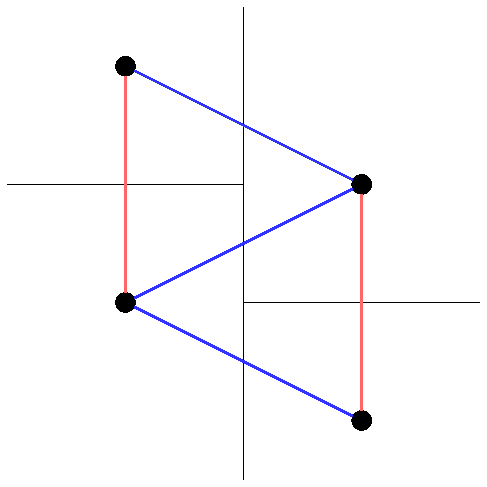
\includegraphics[width=\textwidth]{vertonedsidedalwaysexists1}
        \label{fig:}
    \end{subfigure}
    ~ %add desired spacing between images, e. g. ~, \quad, \qquad, \hfill etc. 
      %(or a blank line to force the subfigure onto a new line)
    \begin{subfigure}[b]{0.45\textwidth}
        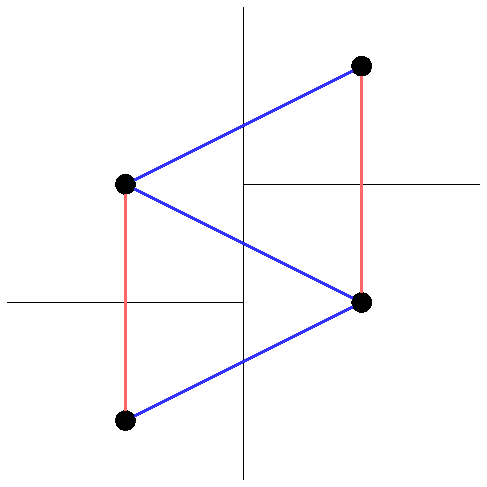
\includegraphics[width=\textwidth]{vertonedsidedalwaysexists2}
    \end{subfigure}
    \caption{ The two cases of Claim 1       \label{fig:vertonedsidedalwaysexists}
}
\end{figure}

\begin{claim}
For every graph $G$ it holds that the horizontally/vertically one-sided segment is the maximal/minimal element in the distributive lattice.
\end{claim}

This claim is false. Consider the graph in figure \ref{fig:disproofhorvertmaxmin}. The rectangular dual corresponding to this graph is vertically one-sided. But this graph contains both left and right-alternating cycles.

\begin{figure}[h!]
\centering
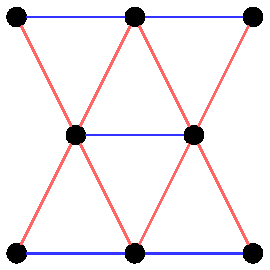
\includegraphics{disproofhorvertmaxmin}

\caption{• 
    \label{fig:disproofhorvertmaxmin}}
\end{figure}

\begin{claim}
All interior edges to a alternating 4cycle inncident to the same vertex have the same color.
\end{claim}

\end{document}